\chapter{Équations de Maxwell et diffraction}
\section{La transformée de Fourier : illustration}
Le but de cette section est d'illustrer l'intérêt de cet transformée. On s'intéressera 
ici au cas de la transformée de Fourier temporelle
\begin{equation}
TF(f) = \int_{-\infty}^\infty f(t)e^{i\omega t}\ dt = F(\omega)
\end{equation}
où le $\omega$ est vu comme la pulsation des composantes harmoniques du signal. Par la 
transformée inverse
\begin{equation}
TF^{-1}(F) = \dfrac{1}{2\pi}\int_{-\infty}^\infty F(\omega)e^{-i\omega t }\ d\omega = f(t)
\end{equation}
qui n'est rien d'autre qu'une somme d'onde d'amplitude $F(\omega)$.\\

On se propose d'étudier la propagation d'impulsions lumineuses en fibre optique. On utilisera 
pour ça un laser de fréquence $\omega_0$ extrêmement élevé monochromatique : si c'est le cas, 
la distribution des fréquences sera un delta de Dirac. Décrivons l'onde électromagnétique de 
la façon suiante
\begin{equation}
E(z,t) = ae^{ik(\omega_0)z}e^{-i\omega_0t}
\end{equation}
où $k$, le nombre d'onde, impose la périodicité spatiale. Quand $z$ progresse de $2\pi/k$, on 
progresse bien d'une période. Si l'on ne regarde pas la dépendance temporelle, on retrouve bien 
le phaseur de l'onde à une dimension. Ce qui est important c'est le nombre d'onde
\begin{equation}
k = k(\omega) = \frac{\omega}{c}n(\omega)
\end{equation}
où $n$ est l'indice de réfraction, dépendant de la dynamique des nuages électroniques. Ce $n
(\omega)$ conditionne la propagation en "cachant" toute la complexité microscopique. En pratique, 
il est intéressant de moduler le faisceau laser de sorte à coder des informations. Le champ 
s'en voit dès lors modulée, l'amplitude devient fonction du temps
\begin{equation}
E(0,t) = a(0,t)e^{-i\omega_0t}
\end{equation}
\begin{center}
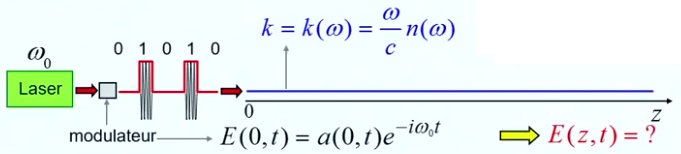
\includegraphics[scale=0.45]{ch2/image1.png}
\captionof{figure}{ }
\end{center}

Ce qui est intéressant est de connaître la sortie du système, que l'on peut considérer comme 
un SLP dont la sortie se trouve en $z$. Introduisons la notion de transformée de Fourier 
temporelle
\begin{equation}
TF(f) = \int_{-\infty}^\infty f(t)e^{i\Omega t}\ dt = F(\Omega)
\end{equation} 
où l'on utilise $\Omega$ car on s'intéresse à la pulsation de l'enveloppe et pas à la 
pulsation rapide $\omega_0$ donnant lieu à cette enveloppe. De même pour la transformée 
inverse
\begin{equation}
TF^{-1}(F) = \dfrac{1}{2\pi}\int_{-\infty}^\infty F(\Omega)e^{-i\Omega t }\ d\omega = f(t)
\end{equation}
Ceci étant fait, on définit le \textbf{spectre} de l'impulsion d'entrée, c'est-à-dire la 
transformée de Fourier suivante
\begin{equation}
A(\Omega) = TF[a(0,t)]
\end{equation}
où
\begin{equation}
a(0,t) = \left\{\begin{array}{ll}
a_0 & \text{ si } |t| \leq T\\
0 & \text{ si } |t| > T
\end{array}\right.\qquad \Rightarrow \quad TF[a(0,t)] = 2a_0T\text{sinc}(\Omega T) = A(\Omega)
\end{equation}
Rappelons qu'une fonction étroite donne une transformée de Fourier large et vice-versa. Nous 
allons maintenant exprimer la fonction comme étant la transformée de Fourier inverse de son 
spectre
\begin{equation}
a(0,t) = TF^{-1}[A(\Omega)]
\end{equation}
Dès lors
\begin{equation}
E(0,t) = \dfrac{1}{2\pi}\int_{-\infty}^\infty A(\Omega)e^{-i\Omega t}\ d\Omega e^{-i\omega_0t}
\end{equation}
En rentrant le facteur exponentiel, il est possible d’interpréter physiquement le résultat
\begin{equation}
E(0,t) = \dfrac{1}{2\pi}\int_{-\infty}^\infty A(\Omega)e^{-i(\omega_0 +\Omega)t}\ d\Omega 
\end{equation}
Le champ à l'entrée de la fibre est donnée par une somme d'onde harmonique dont la pulsation 
n'est plus $\omega_0$ mais $\omega_0+\Omega$ et chacune de ces ondes a une amplitude $A(\Omega)$ 
est donnée par la fonction sinus cardinal qui possède un maximum en $0$.\\

\begin{wrapfigure}[15]{r}{4cm}
\vspace{-5mm}
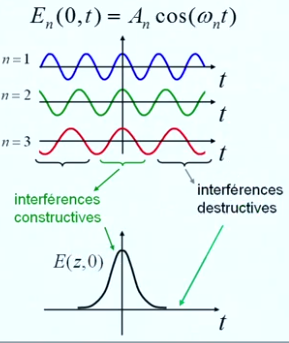
\includegraphics[scale=0.45]{ch2/image2.png}
\captionof{figure}{ }
\end{wrapfigure}
A l'entrée de la fibre, nous retrouvons un \textit{paquet d'onde}. Comment le justifier ? On 
peut intuitivement montré que toute fonction du temps peut être représentée par une 
somme d'onde harmonique (transformée de Fourier inverse). Représentons une somme de cosinus 
d'amplitude différente. A l'origine, les ondes sont en phases sur le maximum. Après un certain 
éloignement, on retrouve des interférences destructives. La combinaison des ondes harmoniques 
peut donner une forme quelconque. Revenons à notre problème physique. 
\begin{equation}
E(0,t) = a(0,t)e^{-i\omega_0t} = \dfrac{1}{2\pi}\int_{-\infty}^\infty A(\Omega)e^{-i(\omega_0
+\Omega)t}\ d\Omega
\end{equation}
La fonction de modulation est donnée par la fonction fenêtre dont nous connaissons la 
transformée de Fourier (sinc). Rappelons qu'une amplitude donnée va bien représenter 
l'amplitude de chacune des ondes harmoniques qui composent le signal. Ceci n'est pas que 
mathématique mais traduit la physique.\\

Notre laser émet des photons à la pulsation $\omega_0$. Ils rentrent dans le modulateur et la 
théorie de Fourier nous dit que oui, la pulsation de l'onde sera changée. Ceci est bien 
physique, il y a réellement une modification de la fréquence du laser\footnote{Ceci se vérifie 
expérimentalement avec un prisme.} $\rightarrow$ l'action du modulateur crée de nouveaux 
photons, une nouvelle distribution d'énergie des photons autour de l'énergie centrale donnée 
par $\hbar\omega_0$. La transformée de Fourier traduit ainsi très bien cette réalité physique.\\

Quel est dès lors le champ pour tout temps, en tout $z$ ? Chaque onde harmonique se propage et 
la façon dont une onde électromagnétique se propage est bien connue : il suffit de rajouter le 
nombre d'onde 
\begin{equation}
E(z,t) =\dfrac{1}{2\pi}\int_{-\infty}^\infty A(\Omega)e^{ik(\omega_0+\Omega)z}e^{-i(\omega_0+\Omega)t}
\ d\Omega
\end{equation}
La seule différence entre cette sortie et l'entrée est un facteur exponentiel correspondant, 
comme vu précédemment, à la \textbf{fonction de transfert} du système. Or, la fonction $k(
\omega_0+\Omega)$ est connu, la fonction de transfert, le \textit{propagateur} est connu. Pour 
tout $z$ on introduit la fonction de transfert qui est un simple facteur de phase qui est connu 
car l'indice de réfraction de la fibre est connue. Simplifions l'expression par son approximation 
au premier ordre
\begin{equation}
k(\omega_0+\Omega) \approx k(\omega_0)+k'(\omega_0)\Omega+\dots\qquad \left(k'=\dfrac{dk}{d\omega}
\right)
\end{equation}
Par substitution
\begin{equation}
E(z,t) =\dfrac{1}{2\pi}\int_{-\infty}^\infty  A(\Omega)e^{i(k_0+k_0'\Omega)z}e^{-i(\omega_0+
\Omega)t}
\ d\Omega
\end{equation}
Sortons tout ce qui ne dépend pas de $\Omega$
\begin{equation}
E(z,t) =\dfrac{1}{2\pi}\int_{-\infty}^\infty  A(\Omega)e^{ik_0'\Omega z}e^{-i\Omega t}\ d\Omega\ \ 
e^{ik_0 z}\ e^{-i\omega_0 t}
\end{equation}
Regroupons les exponentielles
\begin{equation}
E(z,t) =\underbrace{\dfrac{1}{2\pi}\int_{-\infty}^\infty  A(\Omega)e^{i\Omega(t-k_0'z)}\ d\Omega}_{
a(0,t-k_0'z)}\ \ 
e^{ik_0 z}\ e^{-i\omega_0 t}
\end{equation}

\begin{wrapfigure}[7]{l}{6cm}
\vspace{-5mm}
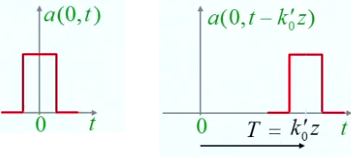
\includegraphics[scale=0.45]{ch2/image3.png}
\captionof{figure}{ }
\end{wrapfigure}
Cette expression n'est que la transformée de Fourier inverse du spectre du modulateur à laquelle 
on rajoute le propagateur de chacune des ondes harmoniques. Dès lors, en "oubliant" le $k_0'z$ 
on reconnaît la transformée inverse. La seule différence avec le signal de départ est une 
translation temporelle de $k_0'z$.
\begin{equation}
E(z,t) = a(0,t-k_0'z)e^{ik_0z}e^{-i\omega_0t}
\end{equation}
En sortie, on retrouvera en $z$ le signal ci-dessus. Ce n'est rien d'autre que le signal d'entrée 
translaté de $k_0'z$. Que représente cette translation? Il se cache la dedans la notion de 
vitesse de groupe. Si le temps $k_0'z$, l'impulsion s'est déplacée de $z$. On peut faire 
apparaître la notion de vitesse de groupe
\begin{equation}
v_g = \dfrac{z}{T} = \dfrac{1}{k_0'} = \left.\dfrac{dk}{d\omega}\right|_{\omega_0}^{-1}
\end{equation}
où $T = k_0'z$ est le temps de propagation. Ce résultat est obtenu par approche au premier 
ordre. Un développement au second ordre mettrait en évidence le phénomène de dispersion.


\newpage
\section{Équation de Maxwell et transformée de Fourier}
































